% 第 1 章 初识 C++
\renewcommand{\codeInset}{63bp}
本章介绍 C++ 的面向对象编程（Object-Oriented Programming，OOP）。我们先研究一个掷骰子的简单程序：编写代码，然后编译、链接并执行程序。

接着构造一个简单的面向对象层次结构，涉及基类 \texttt{Person} 及其两个派生类 \texttt{Student} 和 \texttt{Employee}。我们还会研究指针与动态绑定。

最后，我们创建两个简单的数据类型——栈和队列。栈由自底向上排列的一组值构成，我们只对栈顶的值感兴趣。队列则是传统意义上的值队列：在后端加入值，在前端读取值。

本章将涵盖以下主题：

\begin{itemize}
\item 我们先实现一个简单的游戏：掷骰子。它的主要目的是让你熟悉开发环境，教会你如何建立工程，以及如何编译、链接并执行程序。
\item 然后开始接触面向对象编程：编写一个类层次结构，以 \texttt{Person} 为基类，\texttt{Student} 和 \texttt{Employee} 为派生类。这会介绍继承、封装与动态绑定。
\item 最后，我们为抽象数据类型栈和队列编写类。栈是一种既在顶端加入值、又从顶端移除值的结构；而队列更接近传统意义上的队列：在后端加入值，从前端移除值。
\end{itemize}

\section{掷骰子}

作为入门，我们先编写一个掷骰子的程序。我们使用内置的随机数生成器产生 1 到 6 之间（含两端）的整数值：

\medskip\noindent{\ttfamily\bfseries Main.cpp}

\begin{codebox}
#include <CStdLib>
#include <CTime>
#include <IOStream>
using namespace std;

void main() {
  srand((int) time(nullptr));
  int dice = (rand() % 6 ) + 1;
  cout << "Dice: " << dice << endl;
}
\end{codebox}

在前面的程序中，开头的 include 指令用来包含头文件，头文件里大多存放着标准库的声明。我们需要 \texttt{CStdLib} 头文件来使用随机数生成器，需要 \texttt{CTime} 头文件用当前时间初始化随机数生成器，还需要 \texttt{IOStream} 头文件来输出结果。

标准库存放在名为 \texttt{std} 的命名空间中。命名空间可以看作一个存放代码的容器。我们通过 \texttt{using namespace} 指令获得对标准库的访问。

每个 C++ 程序都有且只有一个 \texttt{main} 函数，程序的执行总是从 \texttt{main} 函数开始。我们用标准函数 \texttt{srand} 和 \texttt{time} 初始化随机数生成器，用 \texttt{rand} 产生实际的随机值。百分号（\texttt{\%}）是取模运算符，它把两个整数相除并给出余数。这样，整型变量 \texttt{dice} 的值就总在 1 到 6 之间。

最后，我们用 \texttt{cout} 输出变量 \texttt{dice} 的值。\texttt{cout} 是标准库用来输出文本和值的对象。

前四章的程序使用 Visual Studio 编写，其余各章的程序则使用 Qt Creator 编写。

下面说明如何创建工程、编写代码并运行应用程序。启动 Visual Studio 后，我们按以下步骤创建工程：

\begin{enumerate}
\item 首先，在 File 菜单中选择 New 和 Project 两个菜单项，如下面的截图所示：
\end{enumerate}

\begin{center}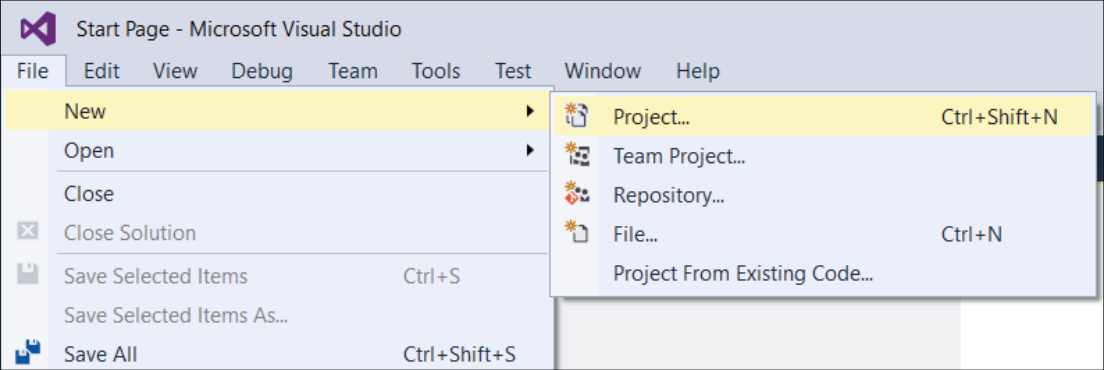
\includegraphics[width=0.85\textwidth]{images/p021_i02.png}\end{center}

\begin{enumerate}\setcounter{enumi}{1}
\item 我们选择 Win32 Console Application 类型，并把工程命名为 Dice：
\end{enumerate}

\begin{center}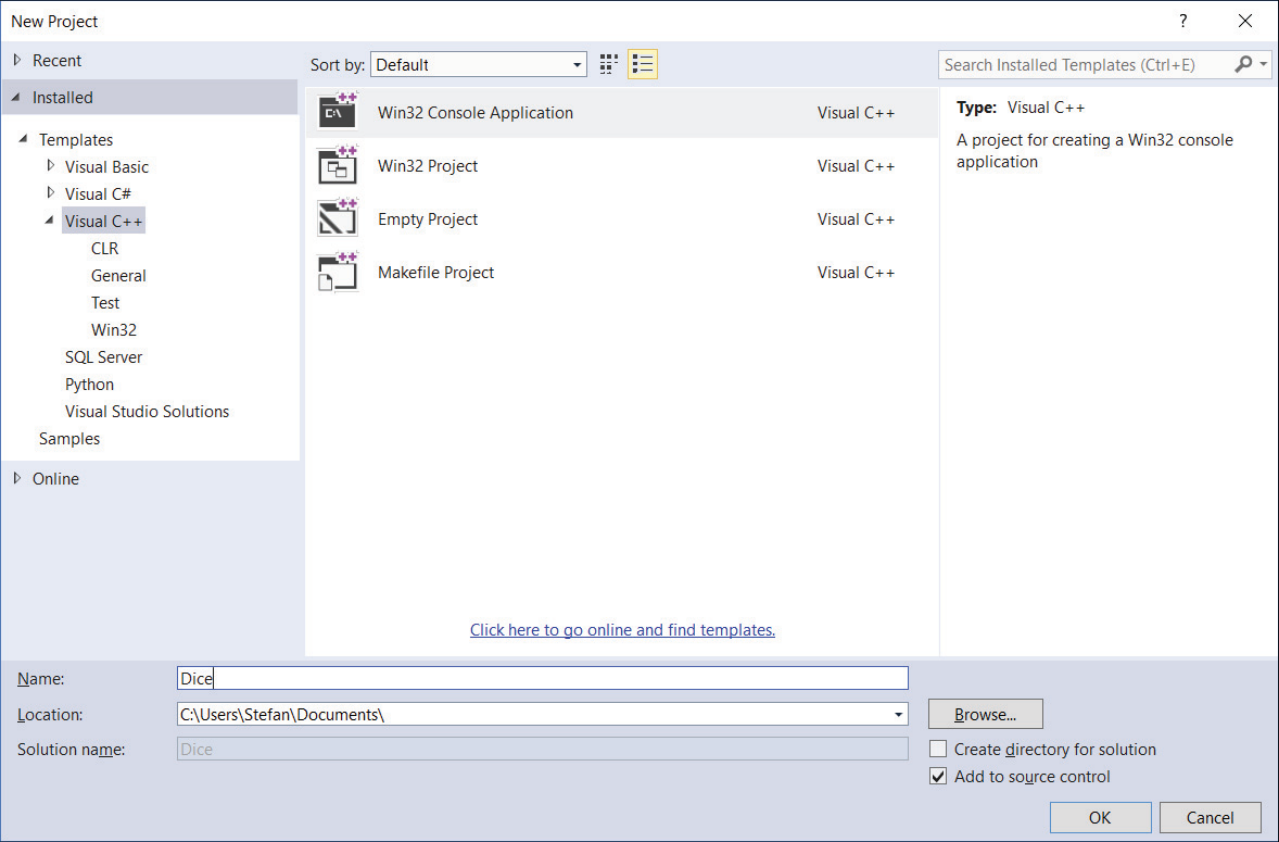
\includegraphics[width=0.98\textwidth]{images/p021_i04.png}\end{center}

\begin{enumerate}\setcounter{enumi}{2}
\item 在第一个对话框中，我们只需按下 Next 按钮：
\end{enumerate}

\begin{center}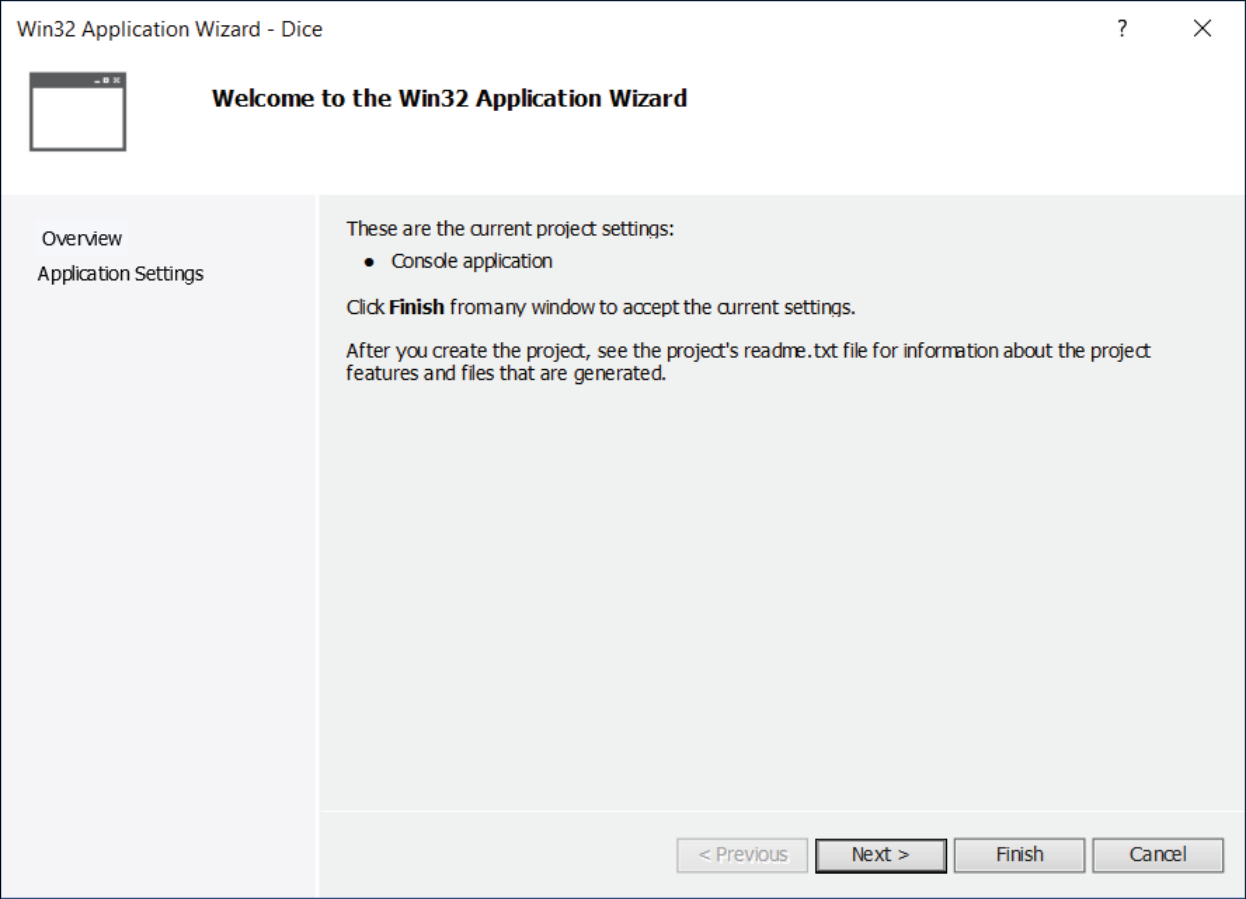
\includegraphics[width=0.95\textwidth]{images/p022_i03.png}\end{center}

\begin{enumerate}\setcounter{enumi}{3}
\item 在第二个对话框中，我们勾选 Empty project 复选框并点击 Finish 按钮。这样将创建一个不含文件的工程：
\end{enumerate}

\begin{center}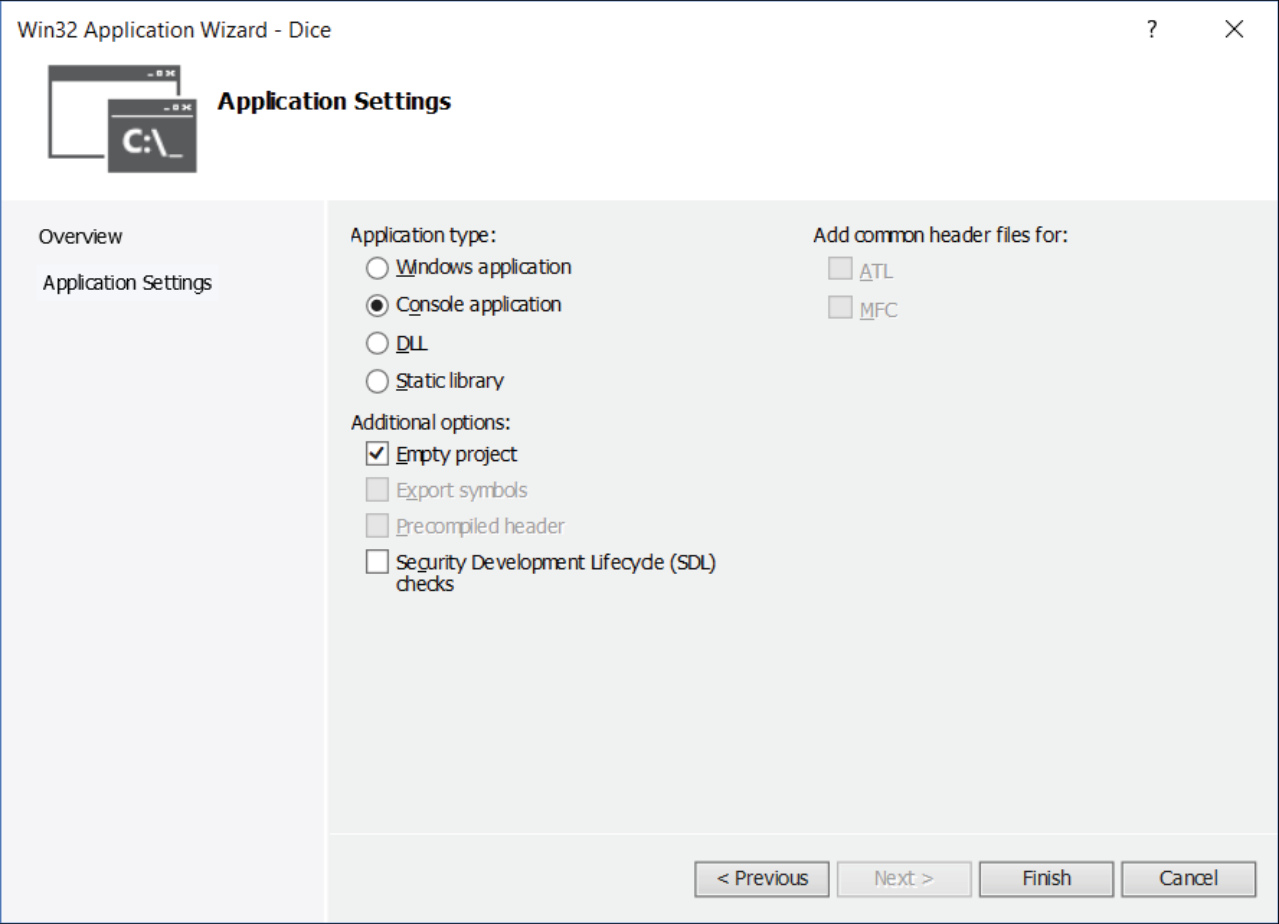
\includegraphics[width=0.95\textwidth]{images/p023_i03.png}\end{center}

\begin{enumerate}\setcounter{enumi}{4}
\item 创建好工程后，我们需要添加一个文件：
\end{enumerate}

\begin{center}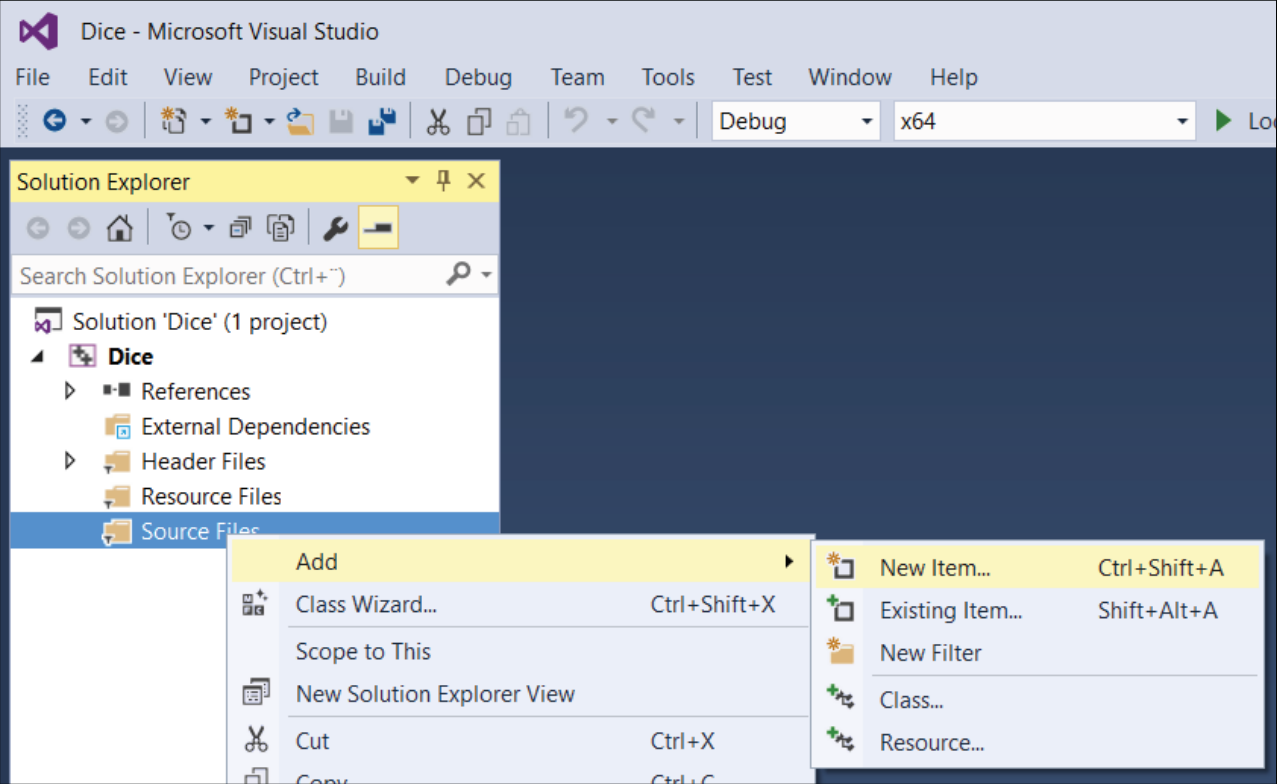
\includegraphics[width=0.98\textwidth]{images/p024_i03.png}\end{center}

\begin{enumerate}\setcounter{enumi}{5}
\item 我们选择 C++ File(.cpp) 类型，并把它命名为 Main.cpp：
\end{enumerate}

\begin{center}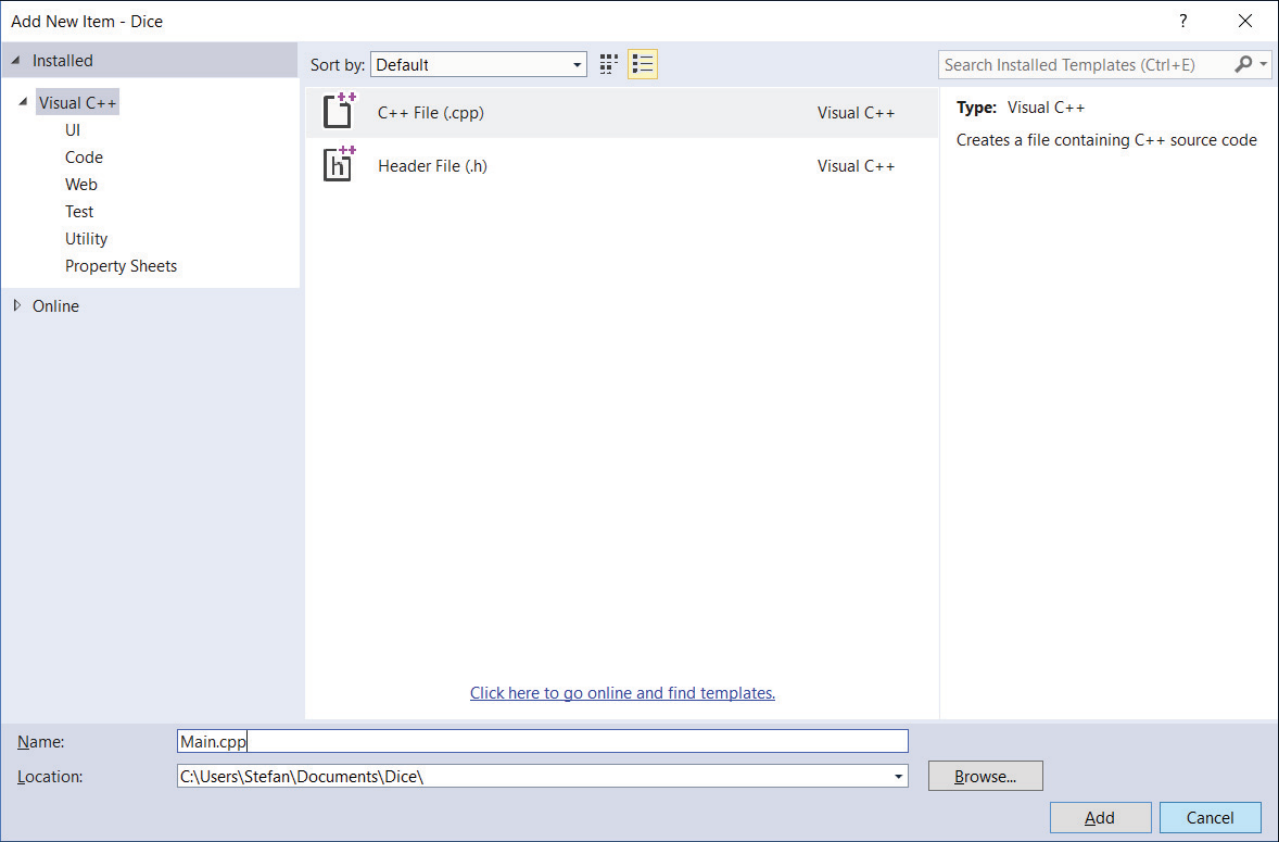
\includegraphics[width=0.95\textwidth]{images/p025_i03.png}\end{center}

\begin{center}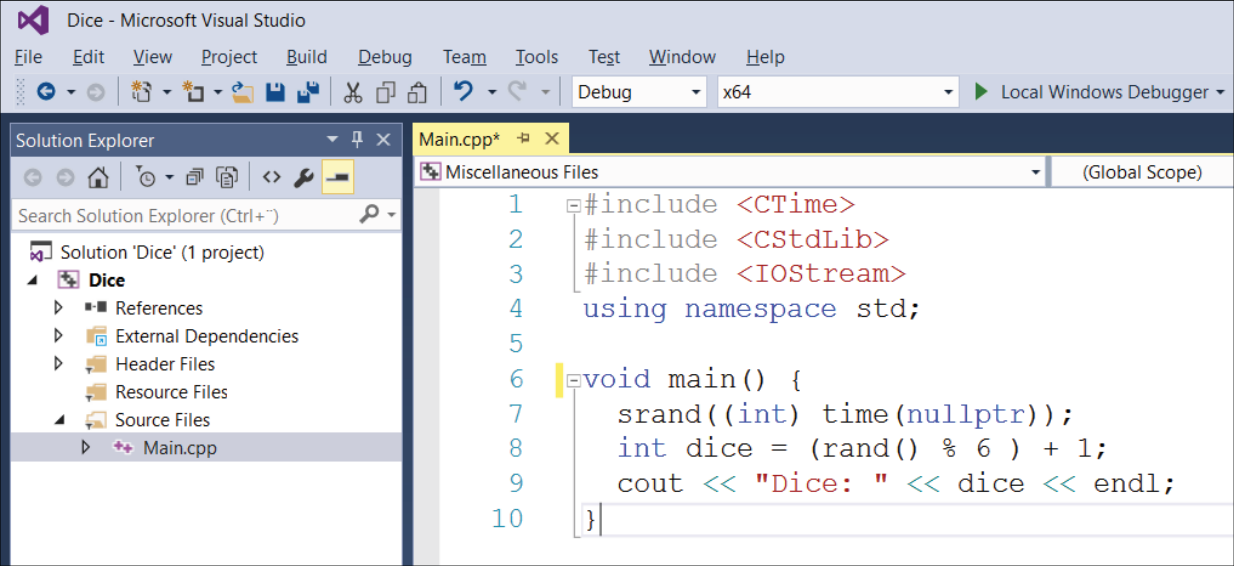
\includegraphics[width=0.95\textwidth]{images/p026_i03.png}\end{center}

\begin{enumerate}\setcounter{enumi}{6}
\item 然后，我们在 Main.cpp 文件中输入代码：
\end{enumerate}

\begin{enumerate}\setcounter{enumi}{7}
\item 最后，我们运行程序。最简单的方法是选择 Start Debugging 或 Start Without Debugging 菜单选项。这样程序就会被编译、链接并执行：
\end{enumerate}

\begin{center}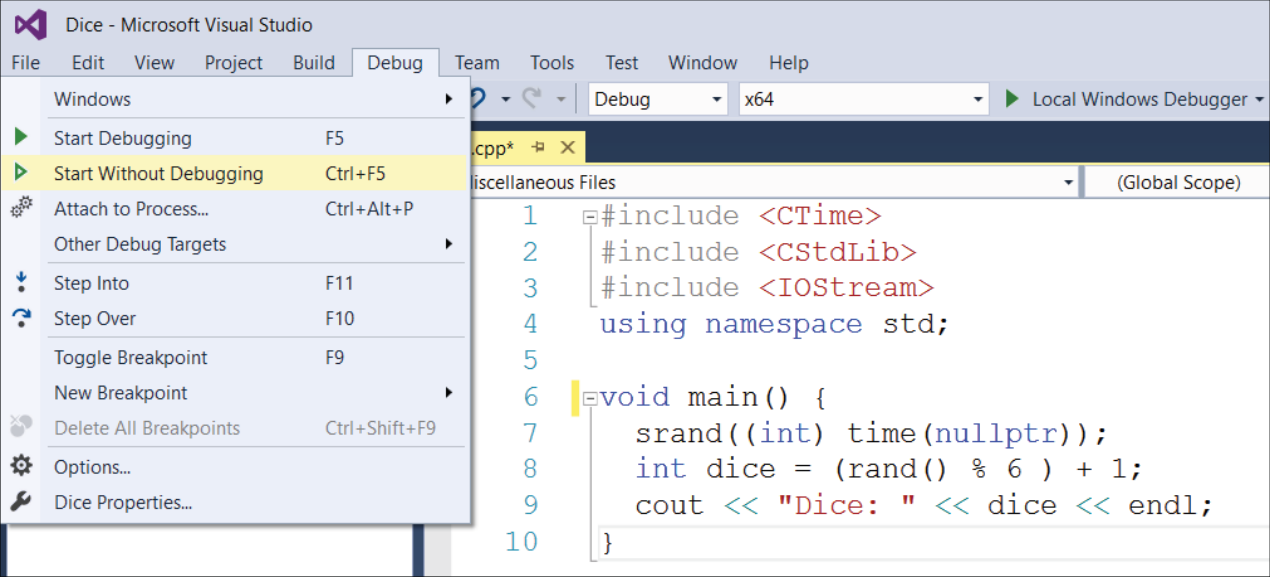
\includegraphics[width=0.98\textwidth]{images/p026_i05.png}\end{center}

\begin{enumerate}\setcounter{enumi}{8}
\item 程序的输出显示在一个命令窗口中：
\end{enumerate}

\begin{center}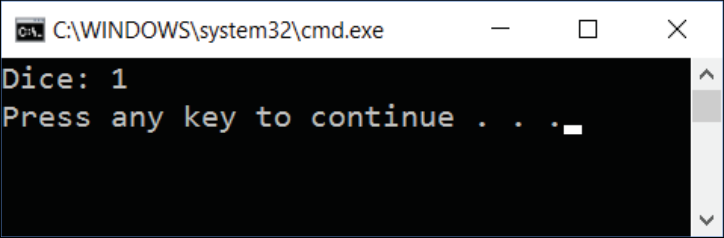
\includegraphics[width=0.55\textwidth]{images/p027_i03.png}\end{center}

\section{理解类 —— Car 类}

我们继续来看一个处理汽车的简单类，包括汽车的速度和方向。类是面向对象语言中一个非常核心的特性。在 C++ 中，类的规格说明由两部分组成——定义与实现。定义部分通常放在头文件（后缀为 \texttt{.h}）中，而实现部分放在后缀为 \texttt{.cpp} 的文件中，如 \texttt{Car.h} 和 \texttt{Car.cpp} 文件。不过，模板类（将在第 3 章「构建图书馆管理系统」中介绍）只存放在一个文件里。

类由其成员组成，成员可以是字段或方法。字段存放某个特定类型的值。方法是一种数学抽象，可以接受输入值并返回一个值。方法的输入值称为参数。不过在 C++ 中，也可以定义没有参数、没有返回类型的函数。

对象是类的实例；同一个类可以创建许多对象。方法可以分为以下几类：

\begin{itemize}
\item \textbf{构造函数}：在对象被创建时调用
\item \textbf{读取器}：读取器读取类的字段
\item \textbf{修改器}：修改器修改字段的值
\item \textbf{析构函数}：在对象被销毁时调用
\end{itemize}

理想情况下，类的方法不应提供对字段的直接访问，否则一旦字段发生变化，方法的名称/类型也得跟着变。方法应当访问的是类的属性。属性是类的概念性要素，未必对应单个字段。类的每个成员都是 public、protected 或 private 的：

\begin{itemize}
\item \textbf{public 成员}：程序的所有其他部分都可以访问。
\item \textbf{protected 成员}：只有它自己的成员或其派生类（下一节介绍）的成员才能访问。
\item \textbf{private 成员}：只有它自己的成员才能访问。但这并不完全成立——类可以邀请其他类成为它的友元（friend），此时后者就能访问它的 private 和 protected 成员。我们将在下一章讨论友元。
\end{itemize}

下面的 \texttt{Car} 类定义有两个构造函数和一个析构函数。在本例中，它们总是与 \texttt{Car} 类同名。析构函数前面带有波浪号（\texttt{\textasciitilde}）。没有参数的构造函数称为默认构造函数。

\begin{myNotic}{p028_i00}{多个方法可以同名，只要它们的参数列表不同即可，这称为重载。更准确地说，这称为上下文无关重载。还有上下文相关重载：两个方法同名且参数列表相同，但返回类型不同。不过，C++ 不支持上下文相关重载。}
\end{myNotic}

因此，一个类可以拥有多个构造函数，只要它们的参数列表不同。但析构函数不允许带参数，所以一个类只能有一个析构函数：

\medskip\noindent{\ttfamily\bfseries Car.h}

\begin{codebox}
class Car {
  public:
    Car();
    Car(int speed, int direction);
    ~Car();
\end{codebox}

\texttt{getSpeed} 和 \texttt{getDirection} 方法是读取器，返回汽车当前的速度和方向。返回值的类型是 \texttt{int}，即整数（integer）的缩写。它们用 \texttt{const} 关键字标记为常量方法，因为它们不修改类的字段。不过，构造函数和析构函数不能是常量的：

\begin{codebox}
    int getSpeed() const;
    int getDirection() const;
\end{codebox}

\texttt{accelerate}、\texttt{decelerate}、\texttt{turnLeft} 和 \texttt{turnRight} 方法是修改器，设置汽车当前的速度和方向。它们会修改类的字段，因此不能标记为常量：

\begin{codebox}
    void accelerate(int speed);
    void decelerate(int speed);
    void turnLeft(int degrees);
    void turnRight(int degrees);
\end{codebox}

\texttt{m\_speed} 和 \texttt{m\_direction} 字段存放汽车当前的速度和方向。前缀 \texttt{m\_} 表示它们是类的成员，而不是方法内的局部变量：

\begin{codebox}
  private:
    int m_speed, m_direction;
};
\end{codebox}

在实现文件中，我们必须包含 \texttt{Car.h} 头文件。\texttt{\#include} 指令属于预处理器的组成部分，它只是把 \texttt{Car.h} 文件的内容包含进来。上一节中我们用尖括号（\texttt{<} 和 \texttt{>}）包含系统文件，而这里我们用引号（\texttt{"}）包含本地文件。系统包含文件（尖括号）包含的是语言本身自带的系统代码，而本地包含文件（引号）包含的是我们自己在工程中编写的代码。从技术上讲，系统包含文件通常从文件系统的某个特殊目录中包含进来，而本地包含文件则通常在文件系统的本地位置包含：

\medskip\noindent{\ttfamily\bfseries Car.cpp}

\begin{codebox}
#include "Car.h"
\end{codebox}

默认构造函数把速度和方向都初始化为 0。冒号（\texttt{:}）记法用来初始化字段。两条斜线（\texttt{//}）与行尾之间的文本称为行注释，会被忽略：

\begin{codebox}
Car::Car()
  :m_speed(0),
   m_direction(0) {
  // Empty.
}
\end{codebox}

第二个构造函数把速度和方向都初始化为给定的参数值：

\begin{codebox}
Car::Car(int speed, int direction)
  :m_speed(speed),
   m_direction(direction) {
  // Empty.
}
\end{codebox}

在前面的构造函数中，其实也可以用赋值运算符（\texttt{=}）代替类初始化记法，如下所示。不过这种写法被认为效率不高，因为代码可以用前面的初始化记法进行优化。注意，赋值时我们用一个等号（\texttt{=}）；比较两个值时，我们用两个等号（\texttt{==}），后者将在第 2 章「数据结构与算法」中介绍：

\begin{codebox}
Car::Car() {
  m_speed = 0;
  m_direction = 0;
}
\end{codebox}

这个类的析构函数什么也不做，包含它只是为了完整起见：

\begin{codebox}
Car::~Car() {
  // Empty.
}
\end{codebox}

\texttt{getSpeed} 和 \texttt{getDirection} 方法只是返回汽车当前的速度和方向：

\begin{codebox}
int Car::getSpeed() const {
  return m_speed;
}

int Car::getDirection() const {
  return m_direction;
}
\end{codebox}

紧跟着等号的加号称为复合赋值运算，它把右边的值加到左边的值上。同样，紧跟着等号的减号把右边的值从左边的值中减去。

斜线（\texttt{/}）后紧跟星号（\texttt{*}）、星号后紧跟斜线之间的文本称为块注释，会被忽略：

\begin{codebox}
void Car::accelerate(int speed) {
  m_speed += speed; /* Same effect as: m_speed = m_speed + speed;
*/
}

void Car::decelerate(int speed) {
  m_speed -= speed;
}

void Car::turnLeft(int degrees) {
  m_direction -= degrees;
}

void Car::turnRight(int degrees) {
  m_direction += degrees;
}
\end{codebox}

现在可以测试我们的类了。为此，我们像在 \texttt{Car.cpp} 文件中那样包含 \texttt{Car.h} 文件，同时还要包含系统头文件 \texttt{IOStream}。和上一节一样，系统头文件用尖括号（\texttt{<} 和 \texttt{>}）括起来。我们还需要使用命名空间 \texttt{std} 来访问其功能：

\medskip\noindent{\ttfamily\bfseries Main.cpp}

\begin{codebox}
#include <IOStream>
using namespace std;
#include "Car.h"
\end{codebox}

在 C++ 中，函数可以属于某个类，也可以不带类而独立存在。类的函数通常称为方法。函数是一种数学抽象，它有输入值（称为参数）并返回一个值。不过在 C++ 中，函数允许没有参数，也可以返回特殊类型 \texttt{void}，表示不返回任何值。

如上一节所述，程序的执行总是从名为 \texttt{main} 的函数开始，而且每个程序必须恰好有一个名为 \texttt{main} 的函数。与其他一些语言不同，文件名不必叫 Main。

不过为方便起见，本书中每个含有 \texttt{main} 函数的文件都命名为 Main.cpp。\texttt{void} 关键字表示 \texttt{main} 不返回值。注意，构造函数和析构函数从不返回值，也不标记 \texttt{void}；而不返回值的其他方法和函数则必须标记 \texttt{void}：

\begin{codebox}
void main() {
\end{codebox}

我们创建一个 \texttt{Car} 类的对象，命名为 \texttt{redVolvo}。对象是类的实例；\texttt{redVolvo} 是众多汽车中的一辆：

\begin{codebox}
  Car redVolvo;
\end{codebox}

输出信息时，我们使用 \texttt{cout} 对象（console output 的缩写），它通常把内容写到文本窗口。由两个左尖括号（\texttt{<<}）组成的运算符称为输出流运算符。\texttt{endl} 指令让下一次输出从下一行的开头开始：

\begin{codebox}
  cout << "Red Volvo Speed: " << redVolvo.getSpeed()
       << " miles/hour" << ", Direction: "
       << redVolvo.getDirection() << " degrees" << endl;
  redVolvo.accelerate(30);
  redVolvo.turnRight(30);
  cout << "Red Volvo Speed: " << redVolvo.getSpeed()
       << " miles/hour" << ", Direction: "
       << redVolvo.getDirection() << " degrees" << endl;
  redVolvo.decelerate(10);
  redVolvo.turnLeft(10);
  cout << "Red Volvo Speed: " << redVolvo.getSpeed()
       << " miles/hour" << ", Direction: "
       << redVolvo.getDirection() << " degrees" << endl;
\end{codebox}

\texttt{blueFiat} 对象是 \texttt{Car} 类的常量对象。这意味着它只能由某个构造函数初始化，之后只能读取而不能修改。更准确地说，只有常量方法才能在常量对象上调用，而只有不修改对象字段的方法才能是常量的：

\begin{codebox}
  const Car blueFiat(100, 90);
  cout << "Blue Fiat Speed: " << blueFiat.getSpeed()
       << " miles/hour" << ", Direction: "
       << blueFiat.getDirection() << " degrees" << endl;
}
\end{codebox}

运行代码后，输出显示在一个命令窗口中：

\begin{center}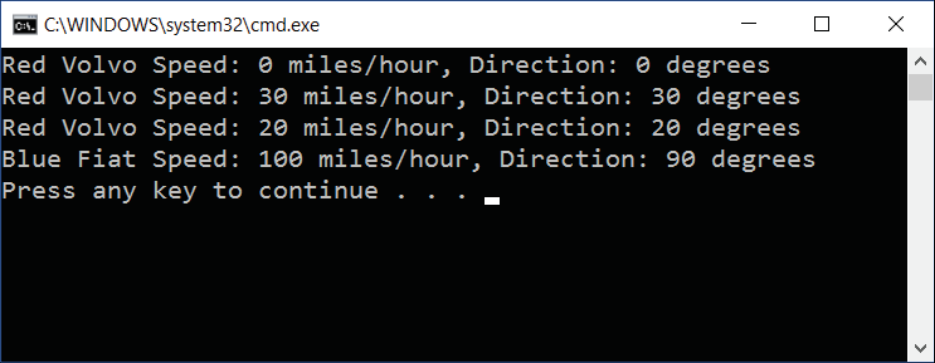
\includegraphics[width=0.72\textwidth]{images/p033_i03.png}\end{center}

\subsection{扩展 Car 类}

本节我们修改 \texttt{Car} 类。在早先的版本中，我们在构造函数里初始化字段。另一种初始化字段的方式是直接在类定义中初始化。不过这一特性应谨慎使用，因为它可能导致不必要的初始化。如果调用的是 \texttt{Car} 类的第二个构造函数，字段就会被初始化两次，效率不高：

\medskip\noindent{\ttfamily\bfseries Car.h}

\begin{codebox}
class Car {
  public:
    // ...
  private:
    int m_speed = 0, m_direction = 0;
};
\end{codebox}

\texttt{Car} 类定义在 \texttt{Car.h} 文件中，而其方法定义在 \texttt{Car.cpp} 文件中。注意我们首先要包含 \texttt{Car.h} 文件，以便方法的定义与 \texttt{Car.h} 中的声明一致：

\medskip\noindent{\ttfamily\bfseries Car.cpp}

\begin{codebox}
#include "Car.h"

Car::Car() {
  // Empty.
}

Car::Car(int speed, int direction)
  :m_speed(speed),
   m_direction(direction) {
  // Empty.
}
\end{codebox}

此外，上一节的 \texttt{Car} 类有一些局限：

\begin{itemize}
\item 可以无限制地加速汽车，而且可以把汽车减速到负速度。
\item 可以把汽车转到方向为负或超过 360 度。
\end{itemize}

我们先把汽车的最大速度设为 200 英里/小时。如果速度超过 200 英里/小时，就把它设为 200 英里/小时。我们使用 \texttt{if} 语句：它接受一个条件，并在条件为真时执行后面的语句。这里的语句（\texttt{m\_speed = 200;}）用花括号括起来。这并非必需，因为只有一条语句；但如果有多条语句就有必要了。为清晰起见，本书中无论语句多少，我们总是使用花括号：

\begin{codebox}
void Car::accelerate(int speed) {
  m_speed += speed;
  if (m_speed > 200) {
    m_speed = 200;
  }
}
\end{codebox}

如果速度变成负值，我们就改变速度的符号使其变为正值。注意，我们不能写 \texttt{m\_speed -= m\_speed}，那会把速度减成零，因为它会从自身中减去自身。

由于值是负的，改变符号后它就变成正值。我们还要把汽车转 180 度来改变方向。注意，这种情况下也必须检查汽车是否超过速度上限。

另外注意，我们还必须检查方向是否小于 180 度。如果是，就加上 180 度；否则减去 180 度，以把方向保持在 0 到 360 度之间。我们用 \texttt{if...else} 语句来做这件事。如果 \texttt{if} 语句的条件不为真，就执行 \texttt{else} 关键字之后的语句：

\begin{codebox}
void Car::decelerate(int speed) {
  m_speed -= speed;
  if (m_speed < 0) {
    m_speed = -m_speed;
    if (m_speed > 200) {
      m_speed = 200;
    }
    if (m_direction < 180) {
      m_direction += 180;
    }
    else {
      m_direction -= 180;
    }
  }
}
\end{codebox}

转动汽车时，我们使用取模（\texttt{\%}）运算符。除以 360 时，取模运算符给出除法的余数。例如，370 除以 360 的余数是 10：

\begin{codebox}
void Car::turnLeft(int degrees) {
  m_direction -= degrees;
  m_direction %= 360;
  if (m_direction < 0) {
    m_direction += 360;
  }
}

void Car::turnRight(int degrees) {
  m_direction += degrees;
  m_direction %= 360;
}
\end{codebox}

\texttt{main} 函数创建一个 \texttt{Car} 类的对象——\texttt{redVolvo}。我们先输出它的速度和方向，然后加速并向左转，再输出速度和方向。最后，减速并向右转，最后一次输出速度和方向：

\medskip\noindent{\ttfamily\bfseries Main.cpp}

\begin{codebox}
#include <IOStream>
using namespace std;
#include "Car.h"

void main() {
  Car redVolvo(20, 30);
  cout << "Red Volvo Speed: " << redVolvo.getSpeed()
       << " miles/hour" << ", Direction: "
       << redVolvo.getDirection() << " degrees" << endl;
  redVolvo.accelerate(30);
  redVolvo.turnLeft(60);
  cout << "Red Volvo Speed: " << redVolvo.getSpeed()
       << " miles/hour" << ", Direction: "
       << redVolvo.getDirection() << " degrees" << endl;
  redVolvo.decelerate(60);
  redVolvo.turnRight(50);
  cout << "Red Volvo Speed: " << redVolvo.getSpeed()
       << " miles/hour" << ", Direction: "
       << redVolvo.getDirection() << " degrees" << endl;
}
\end{codebox}

运行代码后，输出显示在一个命令窗口中，如下所示：

\begin{center}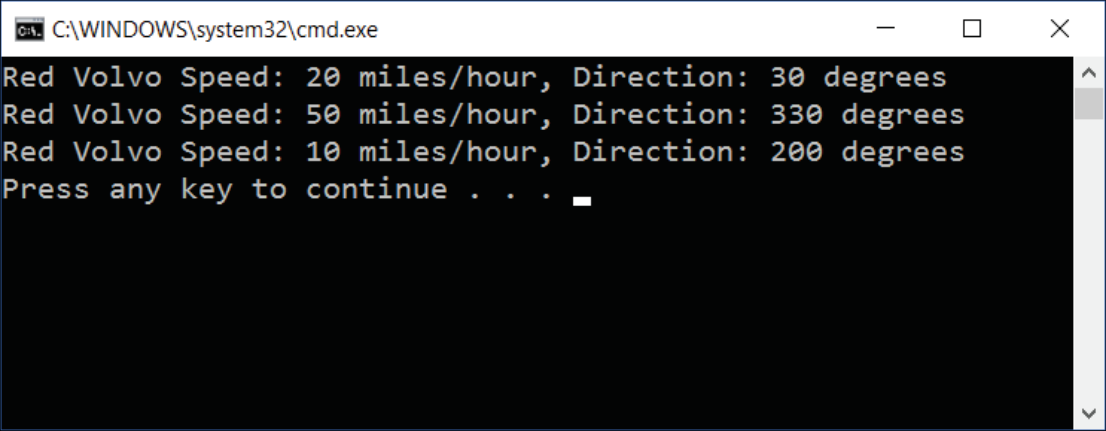
\includegraphics[width=0.85\textwidth]{images/p036_i09.png}\end{center}

\section{类层次结构 —— Person、Student 与 Employee 类}

我们继续看一个类层次结构，其中 \texttt{Person} 是基类，\texttt{Student} 和 \texttt{Employee} 是它的派生类：

\begin{center}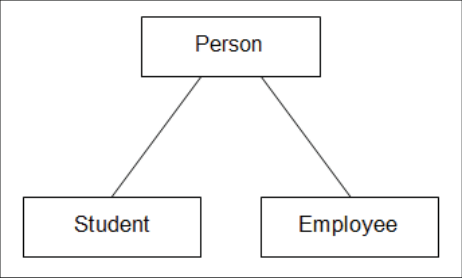
\includegraphics[width=0.38\textwidth]{images/p037_i04.png}\end{center}

由于人有名字，我们使用 C++ 标准类 \texttt{string} 来存放名字。\texttt{virtual} 关键字标记 \texttt{print} 方法将进行动态绑定，本节稍后会讨论：

\medskip\noindent{\ttfamily\bfseries Person.h}

\begin{codebox}
class Person {
  public:
    Person(string name);
    virtual void print();
  private:
    string m_name;
};
\end{codebox}

我们包含 String 头文件，它让我们可以使用 \texttt{string} 类：

\medskip\noindent{\ttfamily\bfseries Person.cpp}

\begin{codebox}
#include <String>
#include <IOStream>
using namespace std;
#include "Person.h"

Person::Person(string name)
  :m_name(name) {
  // Empty.
}

void Person::print() {
  cout << "Person " << m_name << endl;
}
\end{codebox}

\texttt{Student} 和 \texttt{Employee} 类是 \texttt{Person} 的派生类，它们以 public 方式继承 \texttt{Person}。有时人们用「扩展」一词代替「继承」。继承方式可以是 public、protected 或 private 的：

\begin{itemize}
\item public 继承：基类的所有成员对派生类保持相同的可访问性。
\item protected 继承：基类的所有 public 成员在派生类中变为 protected。
\item private 继承：基类的所有 public 和 protected 成员在派生类中变为 private。
\end{itemize}

\texttt{Student} 和 \texttt{Employee} 类有文本字段 \texttt{m\_university} 和 \texttt{m\_company}：

\medskip\noindent{\ttfamily\bfseries Student.h}

\begin{codebox}
class Student : public Person {
  public:
    Student(string name, string university);
    void print();
  private:
    string m_university;
};
\end{codebox}

文件 Student.cpp 定义 \texttt{Student} 类的方法：

\medskip\noindent{\ttfamily\bfseries Student.cpp}

\begin{codebox}
#include <String>
#include <IOStream>
using namespace std;
#include "Person.h"
#include "Student.h"
\end{codebox}

派生类可以通过冒号（\texttt{:}）记法写出基类构造函数的名字来调用基类的构造函数。\texttt{Student} 的构造函数把名字作为参数传给 \texttt{Person} 的构造函数：

\begin{codebox}
Student::Student(string name, string university)
  :Person(name),
   m_university(university) {
  // Empty.
}
\end{codebox}

我们必须用双冒号（\texttt{::}）记法表明调用的是 \texttt{Person} 中的 \texttt{print}，而不是 \texttt{Student} 的：

\begin{codebox}
void Student::print() {
  Person::print();
  cout << "University " << m_university << endl;
}
\end{codebox}

\texttt{Employee} 类与 \texttt{Student} 类似，不过它持有的字段是 \texttt{m\_company} 而不是 \texttt{m\_university}。

\medskip\noindent{\ttfamily\bfseries Employee.h}

\begin{codebox}
class Employee : public Person {
  public:
    Employee(string name, string company);
    void print();
  private:
    string m_company;
};
\end{codebox}

文件 Employee.cpp 定义 \texttt{Employee} 类的方法：

\medskip\noindent{\ttfamily\bfseries Employee.cpp}

\begin{codebox}
#include <String>
#include <IOStream>
using namespace std;
#include "Person.h"
#include "Employee.h"
\end{codebox}

构造函数初始化人名与其供职的公司：

\begin{codebox}
Employee::Employee(string name, string company)
  :Person(name),
   m_company(company) {
  // Empty.
}

void Employee::print() {
  Person::print();
  cout << "Company " << m_company << endl;
}
\end{codebox}

最后，\texttt{main} 函数先包含系统头文件 String 和 IOStream，它们存放着字符串处理以及输入输出流的声明。由于所有标准头文件都在标准命名空间中，我们用 \texttt{using namespace} 指令获得对系统声明的访问：

\medskip\noindent{\ttfamily\bfseries Main.cpp}

\begin{codebox}
#include <String>
#include <IOStream>
using namespace std;
#include "Person.h"
#include "Student.h"
#include "Employee.h"
\end{codebox}

我们定义三个对象 Monica、Demi 和 Charles，并对每个对象调用 \texttt{print}。在这三种情况下，分别调用 \texttt{Person}、\texttt{Student} 和 \texttt{Employee} 类的 \texttt{print} 方法：

\begin{codebox}
void main() {
  Person monica("Monica");
  person.print();
  Student demi("Demi", "MIT");
  student.print();
  Employee charles("Charles", "Microsoft");
  employee.print();
\end{codebox}

星号（\texttt{*}）表示 \texttt{personPtr} 是指向 \texttt{Person} 对象的指针，而不是 \texttt{Person} 对象。指向对象的指针存放的是对象的内存地址，而不是对象本身。不过此刻它根本没有存放任何地址。我们很快会把它赋值为某个对象的地址：

\begin{codebox}
  Person *personPtr;
\end{codebox}

取地址符（\texttt{\&}）是一个运算符，它给出对象的地址，该地址被赋给指针 \texttt{personPtr}。我们依次把 \texttt{Person}、\texttt{Student} 和 \texttt{Employee} 对象的地址赋给 \texttt{personPtr}，并在每种情况下调用 \texttt{print}。由于 \texttt{print} 在 \texttt{Person} 中被标记为 virtual，调用的是指针当前所指向对象所属类中的 \texttt{print}。既然 \texttt{print} 在基类 \texttt{Person} 中被标记为 virtual，就不必在派生类 \texttt{Student} 和 \texttt{Employee} 中再把 \texttt{print} 标记为 virtual。访问指针所指对象的成员时，我们使用箭头（\texttt{->}）运算符，而不是句点运算符。

当 \texttt{personPtr} 指向一个 \texttt{Person} 对象时，调用的是 \texttt{Person} 中的 \texttt{print}：

\begin{codebox}
  personPtr = &person;
  personPtr->print();
\end{codebox}

当 \texttt{personPtr} 指向一个 \texttt{Student} 对象时，调用的是 \texttt{Student} 中的 \texttt{print}：

\begin{codebox}
  personPtr = &student;
  personPtr->print();
\end{codebox}

当 \texttt{personPtr} 指向一个 \texttt{Employee} 对象时，调用的是 \texttt{Employee} 中的 \texttt{print}：

\begin{codebox}
  personPtr = &employee;
  personPtr->print();
}
\end{codebox}

这个过程称为动态绑定。如果我们在 \texttt{Person} 中省略 virtual 标记，就会发生静态绑定，所有情况下调用的都是 \texttt{Person} 中的 \texttt{print}。

面向对象编程的概念建立在三大基石之上：封装、继承和动态绑定。不支持这三个特性中任何一个的语言，都称不上是面向对象的语言。

\section{简单数据类型 —— 栈}

栈是一种简单的数据类型：我们把值加到顶端，移除顶端的值，且只能读取栈顶的值。本节我们实现一个整数栈。下一章我们会研究能存放任意类型值的模板类。我们使用链表——一种让一个指针指向链表的第一个单元格，而每个单元格又持有指向链表中下一个单元格的指针的结构。自然，链表最终必须结束。我们用 \texttt{nullptr} 标记链表的末尾，它是 C++ 中指向特殊空地址的标准指针。

首先，我们需要一个类来存放链表的每个单元格。单元格存放一个整数值和一个指向链表中下一个单元格的指针；如果它是链表的最后一个单元格，则该指针为 \texttt{nullptr}。下面的章节中，我们会研究同时持有前一个和下一个单元格指针的单元格类。

\medskip\noindent{\ttfamily\bfseries Cell.h}

\begin{codebox}
class Cell {
  public:
    Cell(int value, Cell *next);
\end{codebox}

可以直接在类定义中实现方法，这样的方法称为内联方法。不过通常只对短方法这样做。经验法则是：内联方法不应超过一行：

\begin{codebox}
    int value() const { return m_value; }
    Cell *next() const { return m_next; }
\end{codebox}

每个单元格存放一个值和链表中下一个单元格的地址：

\begin{codebox}
  private:
    int m_value;
    Cell *m_next;
};
\end{codebox}

\medskip\noindent{\ttfamily\bfseries Cell.cpp}

\begin{codebox}
#include "Cell.h"
\end{codebox}

单元格用一个值和一个指向链表中下一个单元格的指针来初始化。注意，如果该单元格是链表中最后一个单元格，则 \texttt{m\_next} 的值为 \texttt{nullptr}：

\begin{codebox}
Cell::Cell(int value, Cell *next)
  :m_value(value),
   m_next(next) {
  // Empty.
}
\end{codebox}

对栈来说，我们只对栈顶的值感兴趣。默认构造函数把栈初始化为空。push 在栈顶加入一个值，top 返回栈顶的值，pop 移除栈顶的值，size 返回栈中值的个数，empty 在栈为空时返回 true。\texttt{bool} 类型是一种逻辑类型，可以存放 \texttt{true} 或 \texttt{false} 值。

\medskip\noindent{\ttfamily\bfseries Stack.h}

\begin{codebox}
class Stack {
  public:
    Stack();
    void push(int value);
    int top();
    void pop();
    int size() const;
    bool empty() const;
\end{codebox}

\texttt{m\_firstCellPtr} 字段是指向链表第一个单元格的指针，链表中存放着栈的值。栈为空时，\texttt{m\_firstCellPtr} 将持有 \texttt{nullptr} 值。\texttt{m\_size} 字段存放栈的当前大小：

\begin{codebox}
  private:
    Cell *m_firstCellPtr;
    int m_size;
};
\end{codebox}

包含 CAssert 头文件是为了使用 \texttt{assert} 宏，它用于测试某些条件是否为真。宏是预处理器的一部分，执行特定的文本替换。

\medskip\noindent{\ttfamily\bfseries Stack.cpp}

\begin{codebox}
#include <CAssert>
using namespace std;
#include "Cell.h"
#include "Stack.h"
\end{codebox}

默认构造函数把指向第一个单元格的指针初始化为 \texttt{nullptr}、把大小初始化为零，从而把栈设为空：

\begin{codebox}
Stack::Stack()
  :m_firstCellPtr(nullptr),
   m_size(0) {
  // Empty.
}
\end{codebox}

向栈顶压入新值时，我们用 \texttt{new} 运算符动态分配单元格所需的内存。如果内存耗尽，就返回 \texttt{nullptr}，\texttt{assert} 宏会对它进行测试。如果 \texttt{m\_firstCellPtr} 等于 \texttt{nullptr}，执行将带着错误信息中止。感叹号（\texttt{!}）后跟等号（\texttt{=}）构成不等运算符。两个加号（\texttt{++}）构成自增运算符，表示把值加一。

自增运算符实际上有两个版本——前缀（\texttt{++m\_size}）和后缀（\texttt{m\_size++}）。前缀形式先把值加一再返回新值；后缀形式同样把值加一，但返回的是原值。不过在这里，用哪个版本都没有关系，因为我们只关心结果——\texttt{m\_size} 的值加了一：

\begin{codebox}
void Stack::push(int value) {
  m_firstCellPtr = new Cell(value, m_firstCellPtr);
  ++m_size;
}
\end{codebox}

返回栈顶值之前，必须先检查栈非空，因为返回空栈的栈顶值是不合逻辑的。如果栈为空，执行将带着错误信息中止。单个感叹号（\texttt{!}）是逻辑非运算符。我们返回栈顶的值，它存放在链表的第一个单元格中：

\begin{codebox}
int Stack::top() {
  assert(!empty());
  return m_firstCellPtr->getValue();
}
\end{codebox}

弹出栈顶值时，同样必须检查栈非空。我们把指向链表第一个单元格的指针改为指向下一个单元格。但在此之前，必须先保存第一个指针 \texttt{deleteCellPtr}，以便释放它所指向的单元格的内存。

我们用 \texttt{delete} 运算符释放内存：

\begin{codebox}
void Stack::pop() {
  assert(!empty());
  Cell *deleteCellPtr = m_firstCellPtr;
  m_firstCellPtr = m_firstCellPtr->getNext();
  delete deleteCellPtr;
\end{codebox}

与上面的自增运算符一样，两个减号（\texttt{--}）构成自减运算符，表示把值减一：

\begin{codebox}
  --m_size;
}
\end{codebox}

\texttt{size} 方法只是返回 \texttt{m\_size} 字段的值：

\begin{codebox}
int Stack::size() const {
  return m_size;
}
\end{codebox}

当指向第一个单元格的指针等于 \texttt{nullptr} 时，栈为空。通俗地说，如果指针等于 \texttt{nullptr}，我们就说这个指针是空的：

\begin{codebox}
bool Stack::empty() const {
  return (m_firstCellPtr == nullptr);
}
\end{codebox}

我们通过压入、读取和弹出一些值来测试栈：

\medskip\noindent{\ttfamily\bfseries Main.cpp}

\begin{codebox}
#include <String>
#include <IOStream>
using namespace std;
#include "Cell.h"
#include "Stack.h"

void main() {
  Stack s;
  s.push(1);
  s.push(2);
  s.push(3);
\end{codebox}

打印布尔值时，流运算符输出的不是 true 或 false，而是 true 打印 1、false 打印 0。为了真正打印 true 或 false，我们使用条件运算符。它接受三个值，用问号（\texttt{?}）和冒号（\texttt{:}）分隔。如果第一个值为 true，返回第二个值；如果第一个值为 false，返回第三个值：

\begin{codebox}
  cout << "top " << s.top() << ", size " << s.size()
       << ", empty " << (s.empty() ? "true" : "false") << endl;
  s.pop();
  s.pop();
  s.push(4);
  cout << "top " << s.top() << ", size " << s.size()
       << ", empty " << (s.empty() ? "true" : "false") << endl;
}
\end{codebox}

\section{更高级的数据类型 —— 队列}

队列是传统队列的模型：我们在后端进入值，在前端读取并移除值。还可以知道它容纳的值的个数，以及它是否为空。

与上一节的栈类似，我们用链表实现队列。我们复用 \texttt{Cell} 类；不过对队列来说，我们需要设置单元格的 next 链接。因此，我们把 next 改名为 \texttt{getNext}，并添加新的 \texttt{setNext} 方法：

\medskip\noindent{\ttfamily\bfseries Cell.h}

\begin{codebox}
class Cell {
  public:
    Cell(int value, Cell *next);
    int value() const {return m_value;}
    Cell *getNext() const { return m_next; }
    void setNext(Cell* next) { m_next = next; }
  private:
    int m_value;
    Cell *m_next;
};
\end{codebox}

我们用链表、以与栈类似的方式实现队列。构造函数初始化一个空队列，enter 在队列后端进入一个值，remove 移除队列前端的值，size 返回队列的当前大小，empty 在队列为空时返回 true：

\medskip\noindent{\ttfamily\bfseries Queue.h}

\begin{codebox}
class Queue {
  public:
    Queue();
    void enter(int value);
    int first();
    void remove();
    int size() const;
    bool empty() const;
\end{codebox}

栈的场合我们只对栈顶感兴趣，它存放在链表的开头。队列的场合我们既关心前端也关心后端，这意味着需要访问链表的第一个和最后一个单元格。因此我们有两个指针 \texttt{m\_firstCellPtr} 和 \texttt{m\_lastCellPtr}，分别指向链表中的第一个和最后一个单元格：

\begin{codebox}
  private:
    Cell *m_firstCellPtr, *m_lastCellPtr;
    int m_size;
};
\end{codebox}

\medskip\noindent{\ttfamily\bfseries Queue.cpp}

\begin{codebox}
#include <CAssert>
using namespace std;
#include "Cell.h"
#include "Queue.h"
\end{codebox}

队列创建时是空的：指针为空，大小为零。由于链表中还没有任何单元格，两个单元格指针都指向 \texttt{nullptr}：

\begin{codebox}
Queue::Queue()
  :m_firstCellPtr(nullptr),
   m_lastCellPtr(nullptr),
   m_size(0) {
  // Empty.
}
\end{codebox}

在队列后端进入新值时，我们检查队列是否为空。如果为空，两个指针都指向新单元格。如果不为空，先把最后一个单元格的 next 指针指向新单元格，然后把最后一个单元格指针设为新单元格：

\begin{codebox}
void Queue::enter(int value) {
  Cell *newCellPtr = new Cell(value, nullptr);
  if (empty()) {
    m_firstCellPtr = m_lastCellPtr = newCellPtr;
  }
  else {
    m_lastCellPtr->setNext(newCellPtr);
    m_lastCellPtr = newCellPtr;
  }
  ++m_size;
}
\end{codebox}

\texttt{first} 方法只是返回链表中第一个单元格的值：

\begin{codebox}
int Queue::first() {
  assert(!empty());
  return m_firstCellPtr->value();
}
\end{codebox}

\texttt{remove} 方法让第一个单元格指向第二个单元格。不过首先必须保存它的地址，以便用 C++ 标准的 \texttt{delete} 运算符释放其内存：

\begin{codebox}
void Queue::remove() {
  assert(!empty());
  Cell *deleteCellPtr = m_firstCellPtr;
  m_firstCellPtr = m_firstCellPtr->getNext();
  delete deleteCellPtr;
  --m_size;
}

int Queue::size() const {
  return m_size;
}

bool Queue::empty() const {
  return (m_firstCellPtr == nullptr);
}
\end{codebox}

我们通过进入并移除一些值来测试队列。我们进入值 1、2、3，它们按该顺序排入队列。然后移除前两个值，再进入值 4。此时队列中保存着值 3 和 4：

\medskip\noindent{\ttfamily\bfseries Main.cpp}

\begin{codebox}
#include <CMath>
#include <String>
#include <IOStream>
using namespace std;
#include "Cell.h"
#include "Queue.h"

void main() {
  Queue q;
  q.enter(1);
  q.enter(2);
  q.enter(3);
  cout << "first " << q.first() << ", size " << q.size()
       << ", empty " << (q.empty() ? "true" : "false") << endl;
  q.remove();
  q.remove();
  q.enter(4);
  cout << "first " << q.first() << ", size " << q.size()
       << ", empty " << (q.empty() ? "true" : "false") << endl;
}
\end{codebox}

\section{小结}

本章我们研究了面向对象编程的基础。我们从创建工程、执行掷骰子程序开始。我们还创建了类层次结构，包括基类 \texttt{Person} 及其两个派生类 \texttt{Student} 和 \texttt{Employee}。通过定义指向对象的指针，我们实现了动态绑定。

最后，我们创建了两个数据类型——栈和队列。栈是这样一种结构：我们只关心顶端的值，可以在顶端加入值、读取栈顶值并移除栈顶值。队列则是传统意义上的队列：在后端进入值，在前端读取并移除值。

下一章我们将继续创建数据类型以及更高级的数据类型，如列表和集合。我们还会研究 C++ 的更多高级特性。
